% !TeX program = pdflatex
\documentclass[11pt, a4paper]{article}
\usepackage[a4paper, margin=2.5cm]{geometry}
\usepackage[T1]{fontenc}
\usepackage{lmodern}
\usepackage{amsmath}
\usepackage{graphicx}
\usepackage{url}
\usepackage{subcaption}
\usepackage[spanish,es-noquoting]{babel}
\usepackage{float}

\title{\textbf{Simulación Computacional del Modelo de Ising 2D}}
\author{Análisis de Código}
\date{}

\begin{document}

\maketitle

\section{Fenomenología y Pregunta Física}
El código proporcionado simula el fenómeno del \textbf{ferromagnetismo} mediante el Modelo de Ising bidimensional. En la naturaleza, ciertos materiales (como el hierro o el níquel) presentan una magnetización espontánea a bajas temperaturas, donde los momentos dipolares magnéticos de sus átomos se alinean paralelamente. Sin embargo, cuando el material se calienta por encima de un umbral térmico crítico, conocido como la \textbf{Temperatura de Curie ($T_c$)}, la agitación térmica destruye este ordenamiento a gran escala, y el material experimenta una transición de fase hacia un estado paramagnético (desordenado).

La \textbf{pregunta física principal} que esta simulación busca responder es: \textit{¿Cómo emergen las propiedades macroscópicas termodinámicas (como la magnetización neta, la energía térmica, el calor específico y la susceptibilidad) a partir de las interacciones locales y microscópicas entre espines vecinos sometidos a fluctuaciones térmicas?} Además, el modelo permite estudiar computacionalmente la naturaleza de la transición de fase continua al acercarse a $T_c$.

\section{Modelo Matemático, Variables y Parámetros}
El sistema se modela como una red cuadrada de tamaño $L \times L$, donde cada nodo de la red contiene un espín discreto. 

\subsection*{Variables del Sistema}
\begin{itemize}
    \item $s_{i,j}$: Variable de espín en la posición $(i,j)$ que solo puede tomar dos valores: $+1$ (arriba) o $-1$ (abajo).
    \item $E$: Energía macroscópica total del sistema.
    \item $M$: Magnetización macroscópica total, definida como $M = \sum_{i,j} s_{i,j}$.
\end{itemize}

\subsection*{Parámetros de Control}
\begin{itemize}
    \item $N = L^2$: Número total de espines en la red.
    \item $T$: Temperatura del baño térmico en Kelvin.
    \item $\beta$: Inverso de la temperatura térmica proporcional, $\beta = \frac{1}{k_B T}$ (el código asume $k_B = 1$).
    \item $J$: Constante de acoplamiento de intercambio (asumida positiva para interacciones ferromagnéticas).
    \item $h$: Campo magnético externo.
\end{itemize}

\subsection*{El Hamiltoniano}
La energía total de una configuración microscópica particular está dada por el Hamiltoniano:
\begin{equation}
    H = -J \sum_{\langle ij \rangle} s_i s_j - h \sum_i s_i
\end{equation}
Donde la primera suma ocurre únicamente sobre los pares de primeros vecinos $\langle ij \rangle$ (arriba, abajo, izquierda, derecha). El código implementa \textbf{condiciones de frontera periódicas} (operador módulo \texttt{\% L}) para simular un medio infinito sin efectos de borde.

A partir del muestreo estadístico, se calculan las fluctuaciones para derivar el Calor Específico ($C_v$) y la Susceptibilidad Magnética ($\chi$):
\begin{equation}
    C_v = \frac{\langle E^2 \rangle - \langle E \rangle^2}{N k_B T^2}, \quad \chi = \frac{\langle M^2 \rangle - \langle M \rangle^2}{N k_B T}
\end{equation}

\section{Método Computacional y Justificación Numérica}
\subsection*{El Método Numérico}
El código utiliza un método estocástico de \textbf{Monte Carlo}, específicamente impulsado por el \textbf{Algoritmo de Metropolis}. 

\subsection*{Justificación}
Para calcular las propiedades macroscópicas exactas, la mecánica estadística requiere promediar sobre el ensamble canónico utilizando la Función de Partición $Z = \sum_{\mathcal{C}} e^{-\beta E(\mathcal{C})}$. Para una red de $N$ espines, existen $2^N$ configuraciones posibles. Calcular $Z$ iterando sobre todos los microestados es computacionalmente imposible incluso para redes pequeñas (por ejemplo, para $L=32$, $2^{1024}$ estados). 

El algoritmo de Metropolis resuelve esto mediante un \textbf{muestreo de importancia}. En lugar de visitar todos los estados, el algoritmo propone cambios locales aleatorios y transita hacia nuevos estados con una probabilidad dependiente del cambio de energía local $\Delta E$, favoreciendo los estados más probables (de baja energía) pero permitiendo fluctuaciones térmicas (de alta energía).

La regla de actualización implementada es:
\begin{enumerate}
    \item Seleccionar aleatoriamente un espín $s_{i,j}$.
    \item Calcular el cambio de energía si se invirtiera: $\Delta E = 2 s_{i,j} (J S_{\text{vecinos}} + h)$.
    \item Si $\Delta E \le 0$, el cambio disminuye la energía del sistema y se \textbf{acepta} incondicionalmente.
    \item Si $\Delta E > 0$, el cambio requiere energía térmica y se \textbf{acepta condicionalmente} comparando un número aleatorio uniforme $r \in (0,1)$ con la probabilidad de Boltzmann $P = \exp(-\beta \Delta E)$.
\end{enumerate}

\section{Arquitectura del Programa}
El código está diseñado bajo el paradigma de \textbf{Programación Orientada a Objetos (POO)} en C++, lo que permite una alta modularidad y encapsulamiento.

\subsection*{Clase \texttt{Ising2D}}
Esta clase encapsula tanto los datos como la lógica física del sistema:
\begin{itemize}
    \item \textbf{Estructura de Datos:} La red espacial se almacena utilizando un vector de vectores dinámico bidimensional (\texttt{std::vector<std::vector<int>> spines}).
    \item \textbf{Inicialización (\texttt{Inicie}):} Prepara la red, siembra el generador de números aleatorios (\texttt{std::mt19937}), planta los espines invertidos iniciales indicados por el usuario, y calcula la energía y magnetización iniciales.
    \item \textbf{Núcleo de Cálculo (\texttt{MonteCarlo}):} Representa 1 Paso de Monte Carlo (MCS), ejecutando $N$ intentos consecutivos de inversión de espín seleccionados aleatoriamente espacialmente, lo que constituye una barrida de la red completa.
    \item \textbf{Muestreo Acumulativo (\texttt{Muestreo}):} Una vez que el sistema abandona el estado transitorio (termalización), esta rutina acumula las sumas de energía y magnetización necesarias para calcular promedios, varianzas y observables finales ($C_v, \chi$).
    \item \textbf{Automatización de Visualización:} La clase incluye métodos para generar \textit{scripts} integrados de \texttt{Gnuplot} (\texttt{GenerarScriptTermalizacion}, \texttt{GenerarScriptRed}, etc.). Esto extrae el trabajo de graficación directamente del ejecutable C++, automatizando la creación de gráficas de fase, histogramas y animaciones GIF de los dominios magnéticos.
\end{itemize}

\subsection*{Bucle Principal (\texttt{main.cpp})}
\begin{enumerate}
    \item Solicita parámetros iniciales (tamaño de red, temperatura, espines invertidos).
    \item \textbf{Fase de Termalización:} Ejecuta 5000 MCS descartando las métricas estadísticas finales pero registrando la convergencia al equilibrio térmico. Exporta datos de cómo la red se relaja hacia un estado de menor energía.
    \item \textbf{Fase de Muestreo:} Ejecuta 10000 MCS para la toma de datos de las fluctuaciones en estado de equilibrio y reporta los observables por espín a la terminal.
\end{enumerate}

\section{Experimentos Realizados}

\subsection{Magnetización en Ausencia de Campo Magnético Externo}

Lo más importante del modelo es su predicción de la magnetización de materiales únicamente por la interacción de los spines de los dominios magnéticos y no por influencia de un campo externo.

\begin{table}[H]
    \centering
    \begin{tabular}{|l|r|}
        \hline
        \textbf{Parámetro} & \textbf{Valor} \\
        \hline
        $h$ (J) & 0 \\
        $N$ & 2500 \\
        Spines Iniciales & 1250 \\
        Temperatura(K) & 1 \\
        \hline
    \end{tabular}
    \caption{Parámetros iniciales de la simulación.}
    \label{tab:parametros-simulacion}
\end{table}

A temperaturas menores a la Temperatura de Curie $T_c$ se puede generar dicha magnetización espontánea por la alineación de los spines. A continuación se muestran 3 momentos de la red durante el proceso de termalización.

\begin{figure}[H]
    \centering
    \begin{subfigure}[t]{0.33\textwidth}
        \centering
        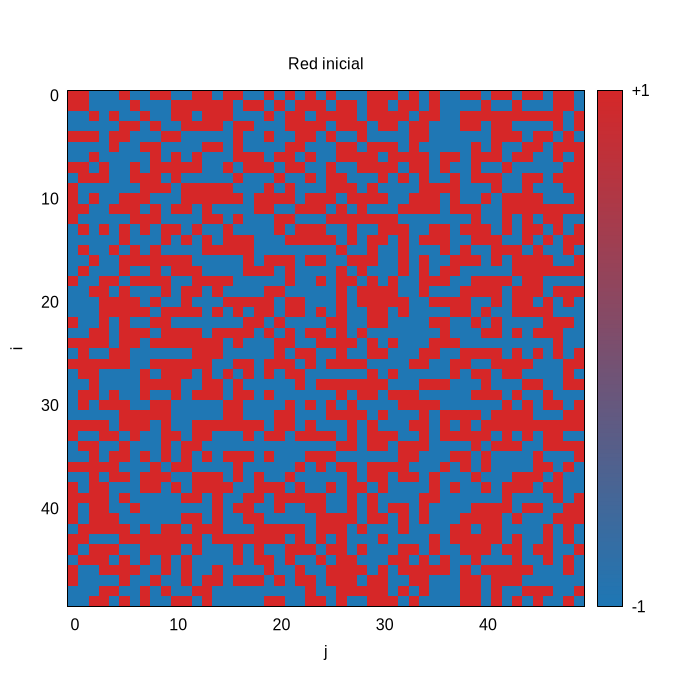
\includegraphics[width=\linewidth]{imagenes/im1.png}
        \caption{Red inicial}
        \label{fig:red-inicial}
    \end{subfigure}\hfill
    \begin{subfigure}[t]{0.30\textwidth}
        \centering
        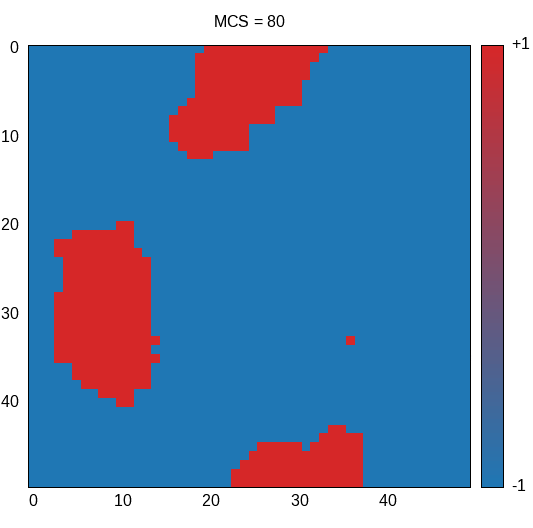
\includegraphics[width=\linewidth]{imagenes/im3.png}
        \caption{Red en el MCS 80}
        \label{fig:red-mcs-80}
    \end{subfigure}\hfill
    \begin{subfigure}[t]{0.33\textwidth}
        \centering
        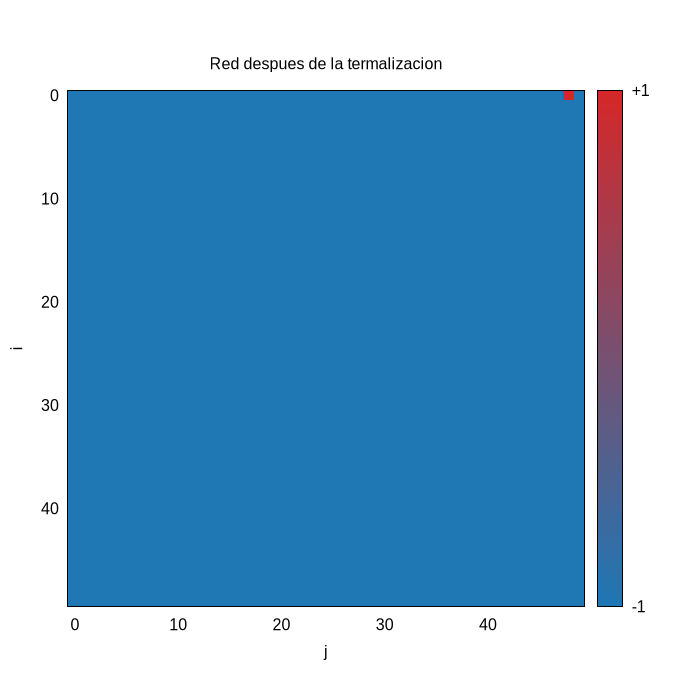
\includegraphics[width=\linewidth]{imagenes/im2.png}
        \caption{Red final}
        \label{fig:red-final}
    \end{subfigure}
    \caption{Evolución de la red durante la termalización.}
    \label{fig:evolucion-red}
\end{figure}

\subsubsection{Evolución de la Energía del sistema}

El sistema parte desde la energía inicial y durante la termalización rápidamente salta a un estado de menor energía (todos los spines alineados, en este caso en -1). Posteriormente se queda oscilando al rededor de ese valor, ya que el sistema permite pequeñas fluctuaciones por agitaciones térmicas en la dirección de los spin.

\begin{figure}[H]
    \centering
    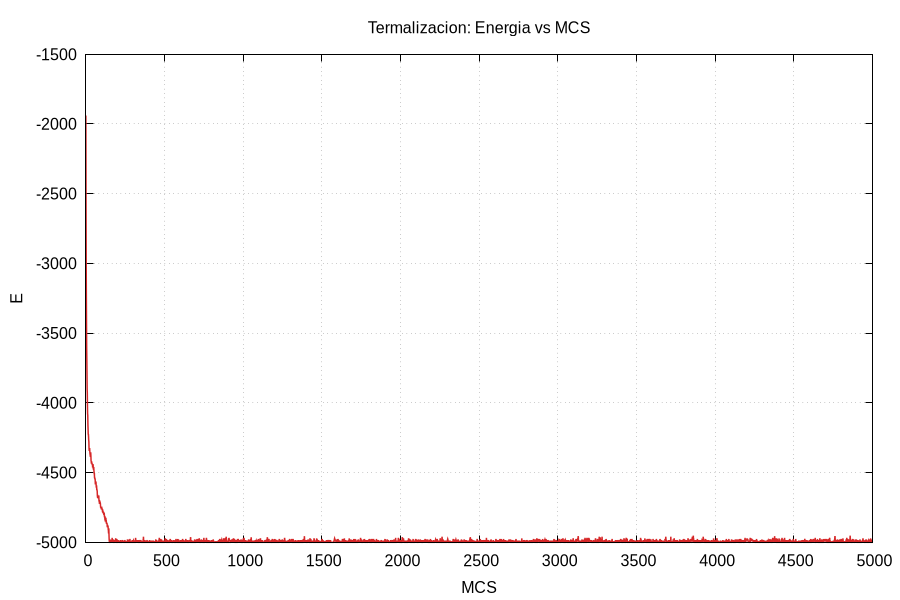
\includegraphics[width=0.8\textwidth]{imagenes/im4.png}
    \caption{Evolución de la energía durante los MCS}
    \label{fig:example_image}
    
\end{figure}

\subsubsection{Evolución de la Magnetización del sistema}

El sistema parte desde una magnetización 0, pues en el estado inicial el numero de spines en -1 y +1 es igual, teniendo un comportamiento paramagnético donde la magnetización de cada spin se cancela entre sí. Rápidamente el sistema pasa a una magnetización negativa correspondiente al número total de partículas y oscila al rededor debido a las agitaciones térmicas.

\begin{figure}[H]
    \centering
    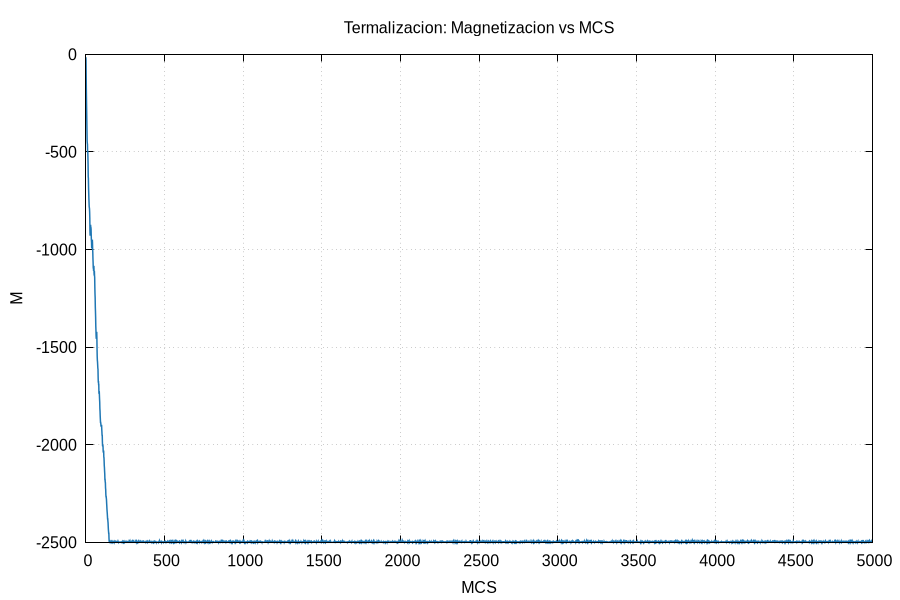
\includegraphics[width=0.8\textwidth]{imagenes/im5.png}
    \caption{Evolución de la magnetización durante los MCS}
    \label{fig:example_image}
    
\end{figure}

\subsubsection{Evolución del número de spines en -1 en el sistema}

El sistema parte desde 1250 según lo ingresado por el usuario, y posteriormente debido a la interacción con los demás constituyentes del sistema, el número empieza a aumentar hasta llegar 2500 que corresponde a $N$ y oscila al rededor de este valor por agitaciones térmicas.

\begin{figure}[H]
    \centering
    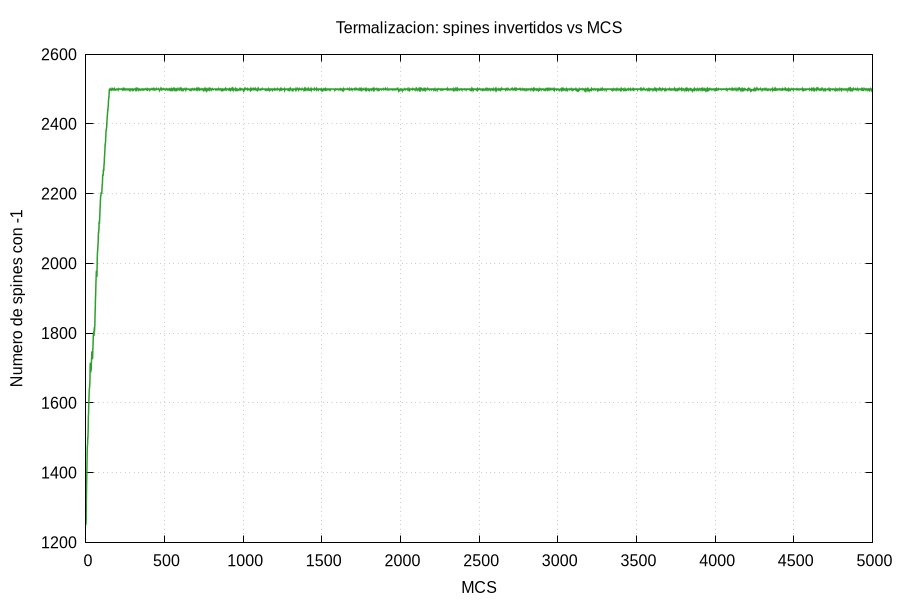
\includegraphics[width=0.8\textwidth]{imagenes/im6.png}
    \caption{Evolución del número de spines invertidos durante los MCS}
    \label{fig:example_image}
    
\end{figure}

\subsection{Ausencia de Magnetización Espontánea para $T>T_c$}

Cuando el sistema se encuentra por encima de la Temperatura de Curie ($2.26919K$), la agitación térmica de los spines no permite que se genere magnetización, manteniendo el sistema en desorden.

\begin{table}[H]
    \centering
    \begin{tabular}{|l|r|}
        \hline
        \textbf{Parámetro} & \textbf{Valor} \\
        \hline
        $h$ (J) & 0 \\
        $N$ & 2500 \\
        Spines Iniciales & 1250 \\
        Temperatura(K) & 3 \\
        \hline
    \end{tabular}
    \caption{Parámetros iniciales de la simulación.}
    \label{tab:parametros-simulacion}
\end{table}

\begin{figure}[H]
    \centering
    \begin{subfigure}[t]{0.5\textwidth}
        \centering
        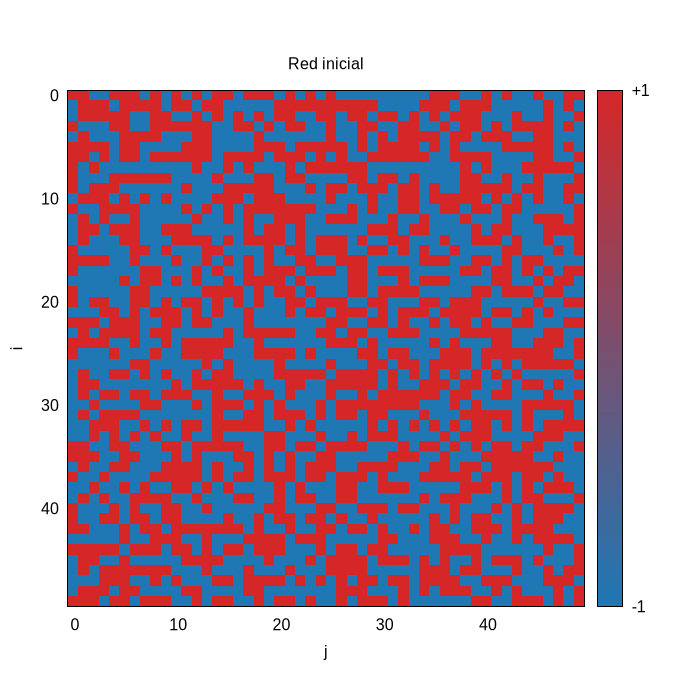
\includegraphics[width=\linewidth]{imagenes/im7.png}
        \caption{Red inicial}
        \label{fig:red-mcs-80}
    \end{subfigure}\hfill
    \begin{subfigure}[t]{0.5\textwidth}
        \centering
        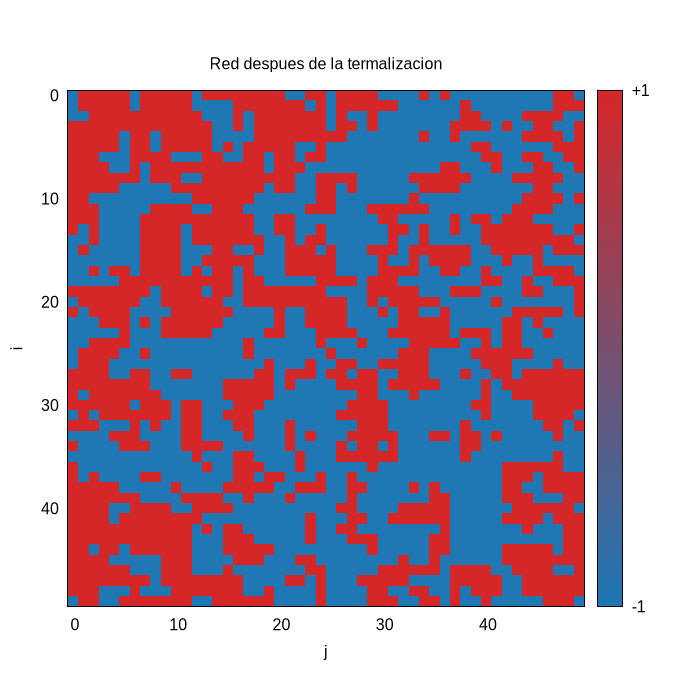
\includegraphics[width=\linewidth]{imagenes/im8.png}
        \caption{Red final}
        \label{fig:red-final}
    \end{subfigure}
    \caption{Evolución de la red durante la termalización.}
    \label{fig:evolucion-red}
\end{figure}

\subsubsection{Evolución de la Energía}

\begin{figure}[H]
    \centering
    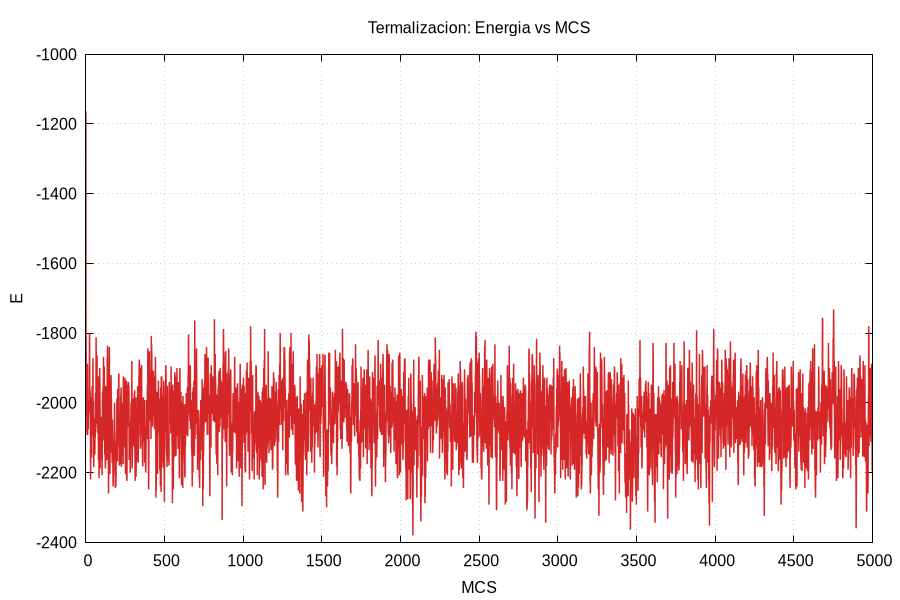
\includegraphics[width=0.8\textwidth]{imagenes/im9.png}
    \caption{Evolución de la energía durante los MCS}
    \label{fig:example_image2}
    
\end{figure}

\subsubsection{Evolución de la Magnetización}

\begin{figure}[H]
    \centering
    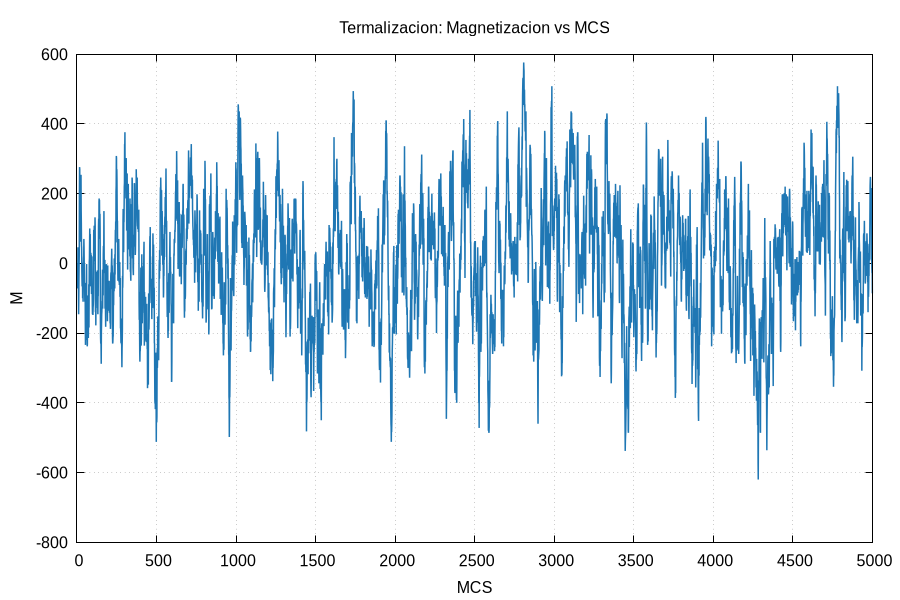
\includegraphics[width=0.8\textwidth]{imagenes/im10.png}
    \caption{Evolución de la magnetización durante los MCS}
    \label{fig:example_image3}
    
\end{figure}

\subsubsection{Evolución de los spines invertidos}

\begin{figure}[H]
    \centering
    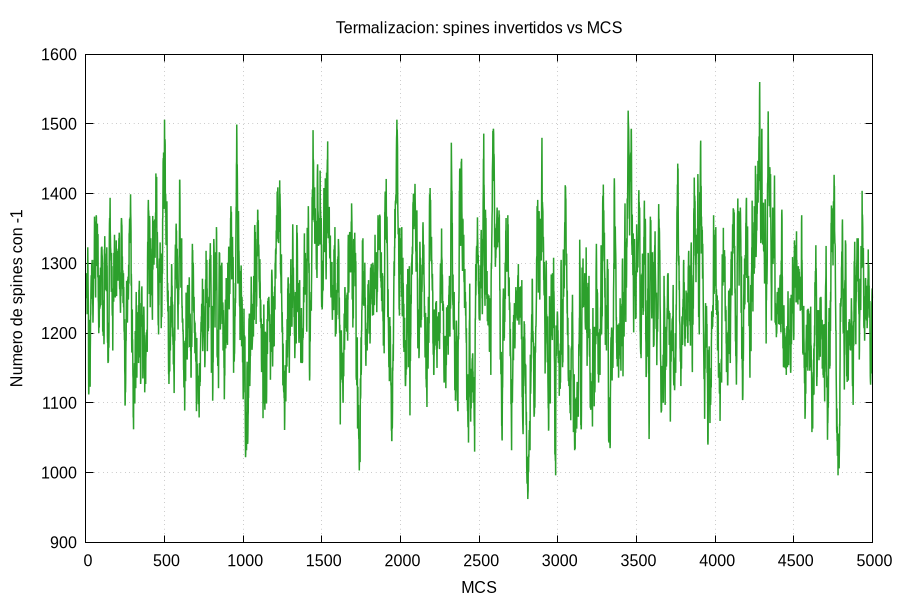
\includegraphics[width=0.8\textwidth]{imagenes/im11.png}
    \caption{Evolución del número de spines invertidos durante los MCS}
    \label{fig:example_image3}
    
\end{figure}

Como se puede observar en las 3 gráficas, en general el sistema se queda oscilando al rededor de su estado inicial. Las fluctuaciones térmicas no permiten que este alcance un estado más ordenado.

El único caso diferente es para la energía, la cual debido a la naturaleza del modelo transita rápidamente a un estado de menor energía no muy alejado del inicial. En la red esto se manifiesta como una formación de "islas" de spines, una distribución espacial de menor energía. Sin embargo la proporción entre spines en -1 y +1 se mantiene similar.

\subsection{Calor Específico y Suceptibilidad Magnética}

Estos dos observables poseen un comportamiento similar:
\begin{itemize}
    \item \textbf{Calor específico ($C_v$):} Para temperaturas inferiores a $T_c$, al aumentar la temperatura crecen las fluctuaciones de energía y, con ellas, el calor específico. Este aumenta hasta divergir en $T_c$. Por encima de $T_c$, el sistema entra en régimen paramagnético y el calor específico disminuye.
    \item \textbf{Susceptibilidad magnética ($\chi$):} Mide la respuesta de la magnetización ante un campo magnético externo. A bajas temperaturas, predominan las interacciones entre espines y el sistema es rígido, por lo que la susceptibilidad es baja. Al acercarse a $T_c$, la agitación térmica aumenta la susceptibilidad hasta divergir. Para $T>T_c$, el desorden térmico reduce la respuesta magnética y la susceptibilidad disminuye.
\end{itemize}

\begin{table}[H]
    \centering
    \begin{tabular}{|c|r|r|}
        \hline
        \textbf{Temperatura (K)} & \textbf{$C_v$} & \textbf{$\chi$} \\
        \hline
        $0.5$ & $3.07 \times 10^{-5}$ & $9.59 \times 10^{-7}$ \\
        $T_c = 2.26919$ & 2.207 & 23.318 \\
        $8$ & 0.034 & 0.223 \\
        \hline
    \end{tabular}
    \caption{Calor específico y susceptibilidad magnética para distintas temperaturas.}
    \label{tab:observables-temperatura}
\end{table}

\section{Conclusiones}

La simulación del modelo de Ising bidimensional con $N=2500$ espines y campo externo nulo muestra cómo las interacciones locales, muestreadas mediante el algoritmo de Metropolis, producen comportamientos macroscópicos distintos según la temperatura. Para $T<T_c$, la red tiende a ordenarse y presenta magnetización espontánea; para $T>T_c$, las fluctuaciones térmicas mantienen una configuración desordenada y reducen la magnetización neta.

Los valores calculados de $C_v$ y $\chi$ son mayores cerca de la temperatura crítica ($T_c=2.26919$) que a $T=0.5$ y $T=8$, lo que indica una respuesta más intensa del sistema en esa región. En conjunto, los resultados ilustran la transición entre los regímenes ferromagnético y paramagnético y muestran cómo los observables termodinámicos reflejan los cambios en la organización de los espines.


\renewcommand{\refname}{Referencias}
\nocite{marenduzzo_mvp}
\bibliographystyle{plainurl}
\bibliography{referencias}

\end{document}
